We also use \texttt{BAFFLES} to derive age posteriors from calcium H (3968.47 \r{A}) and K (3933.67 \r{A}) emission ($R'_{HK}$) for stars with spectral types between F5 and K2. $R'_{HK}$ is derived from the S-value index, which is the ratio of calcium emission flux to nearby continuum. S-values were initially measured photometrically following the methods of the Mt. Wilson Ca II H \& K survey that ran from 1966 to 1983 \citep{1991ApJS...76..383D}. The emission flux is measured through two triangular bandpasses, and the continuum flux is measured through two rectangular bandpasses on either side of the emission cores, as shown in Figure \ref{RHK_examples}. 

\begin{figure*}[ht !]
\centering
 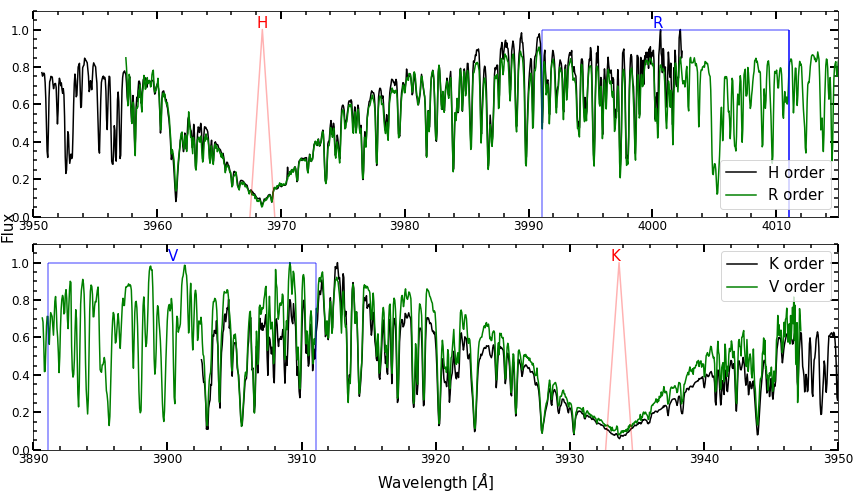
\includegraphics[scale = 0.4]{RHK_ex_HIP102040.png}
 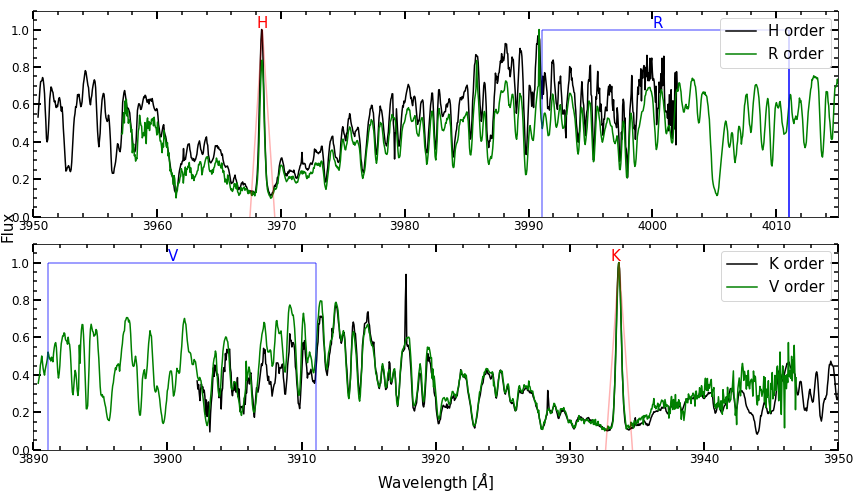
\includegraphics[scale = 0.4]{RHK_ex_HIP115147.png}
 \caption{\rev{The S-value is measured from spectra using triangular transmission profiles (red lines) centered on the Ca II H and K emission lines, and rectangular profiles (blue lines) to measure the nearby continuum level. The top two panels show an example of a low-activity star with no significant H and K emission (HIP 102040), and the bottom two panels show HIP 115147, a star with strong H and K emission.}}
 \label{RHK_examples}
\end{figure*}


Subsequently, the photometric S-value index is most commonly measured from spectra with the S-value index calibrated for each instrument. To calibrate APO/ARCES, we observe 99 stars with published S-values from \cite{2013A&A...551L...8P}, which compiled published S-values from the literature including \cite{1991ApJS...76..383D}, \cite{2004ApJS..152..261W}, and \cite{2003AJ....126.2048G}. We follow a prescription similar to that in \cite{2004ApJS..152..261W} with some modifications to calibrate the APO S-values. \rev{We use a 1-parameter fit (compared to the 4-parameter fit of \rev{\citealt{2004ApJS..152..261W})} with the form \begin{equation}\label{eq:s}
 S = a\left(\frac{H+K}{R+V}\right)
\end{equation}}
%A star's calcium emission traces chromospheric activity and can vary with time over the stellar cycle. \rev{We select stars with more than one reported S-value measurement, and we take the median S-value as our calibration reference.}
$H$ and $K$ are the summed counts from convolving the spectrum with the triangular transmission profiles, while $R$ and $V$ are the summed counts from convolving the continuum with the rectangular transmission profiles (taken from \rev{\citealt{1991ApJS...76..383D})}.

 \rev{We shift the spectra to the rest frame so the calcium emission cores or the centers of the absorption lines are centered in the narrow triangular band passes. Using the $G_{BP}-G_{RP}$ to $B-V$ conversion described in Section \ref{sec:data}, and the grid from \cite{2013ApJS..208....9P} we find effective temperatures, masses, and radii for our targets, assuming they are on the main sequence. We find the synthetic spectrum with solar metallicity from \cite{2013A&A...553A...6H} with the closest effective temperature and surface gravity. We convolve the synthetic spectrum with a Gaussian to match the resolution of ARCES. Then, we shift the ARCES spectra to the rest frame by cross correlating the observed spectrum with the theoretical spectral template.}
 

\rev{Literature S-values are often not given with error bars, and generally variation over the star's activity cycle is expected to be larger than measurement errors. Given the lack of reliable error bars we do not attempt to derive a posterior probability distribution on the fit parameter. Instead, we assume error bars of unity for each measurement, and find the value of $a$ in Equation \ref{eq:s} that minimizes the $\chi^2$. We compute this minimum value over a uniform grid for $a$ with $10^6$ elements between 0 and 40, finding a best-fit value of $a = 18.3$, which results in a $\sim$15\% scatter on the relationship between APO S-values and the literature S-values. The fit is shown in Figure \ref{sval_calib}, and we attribute this $\sim$15\% scatter mainly to variable emission over a stellar cycle.}


\rev{We investigated more complicated fits, such as including additional parameters to weight the H and K bands or the R and V bands differently, or attempting to further correct the continuum by comparing to theoretical spectra, or performing different fits for different spectral type bins. None of these more complicated methods significantly improved the scatter, and some resulted in systematic offsets from the fit at larger S-values. As a result, we adopt the more straightforward approach outlined above.}


\begin{figure*}[ht!]
\centering
  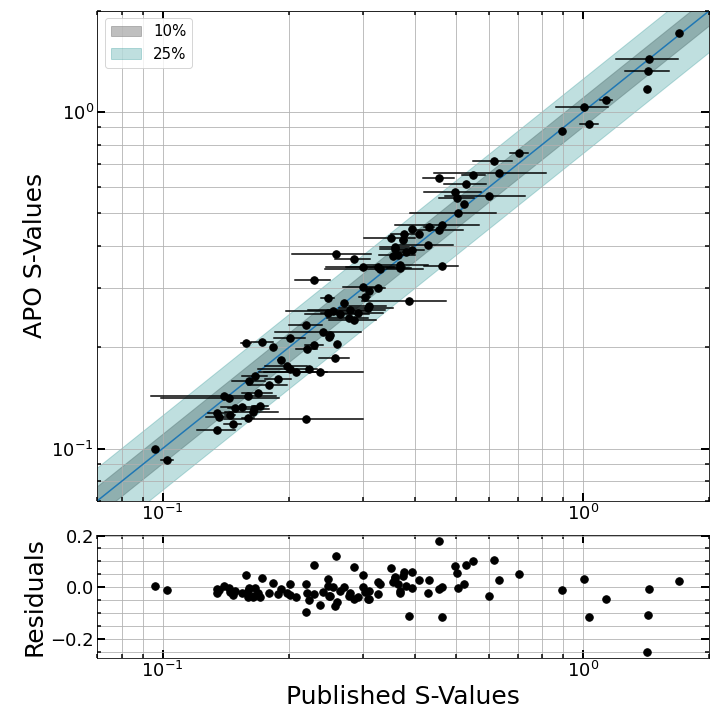
\includegraphics[scale = 0.5]{s_vals_1param.png}
 
 \caption{\rev{We use a 1 parameter fit to calibrate chromospheric S-values from APO/ARCES to values reported in the literature. We observe a  $\sim15\%$ scatter in the relationship, which we largely attribute to the intrinsic variability in chromospheric activity for each star. Error bars represent the maximum and minimum S-value reported in the literature for each star. We report S-values and $log(R'_{HK})$ for all the accelerating stars in Table \ref{tab:rhk}.}}
 \label{sval_calib}

\end{figure*}




The transformation from S-value to $R'_{HK}$  is \begin{equation}\label{eq:r}
R'_{HK} = 1.34\times10^{-4}C_{Cf}S - R_{phot}
\end{equation} \noindent where $C_{Cf}$ is the color correction factor, a third-order polynomial in $B-V$  \citep{1982PhDT.......153M}, and $R_{phot}$ is another third-order polynomial in $B-V$ that corrects for the photospheric contribution to the emission in the Ca H and K lines \citep{1984ApJ...276..254H}. 
\begin{figure*}[ht!]
\centering
  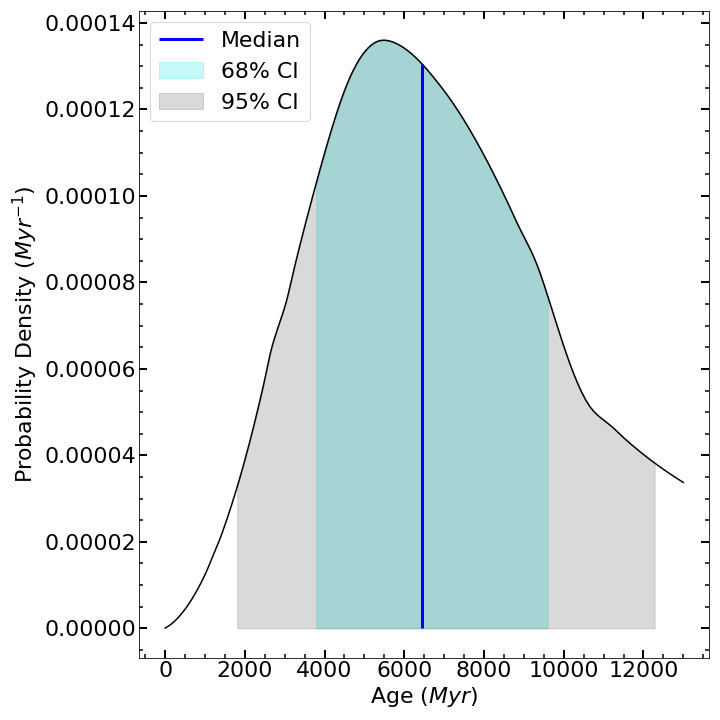
\includegraphics[scale = 0.375]{example_Ca_post.png}
 
 \caption{An example age posterior for HIP 669, using our APO/ARCES measurement and \texttt{BAFFLES} \citep{2020ApJ...898...27S}. For this relatively inactive star, with $log(R'_{HK}) = -4.88$ and $B-V=0.62\pm0.015$, we derive an age posterior with a median age of 6.5 Gyr and $68\%$ confidence interval between 3.8 and 9.7 Gyr.}
 \label{RHK_post_example}

\end{figure*}
S and $R'_{HK}$ are given for each of our target stars in Table \ref{tab:rhk}, as well as \rev{median ages and $68\%$ and $95\%$ confidence intervals} for the 34 stars between F5 and K2 derived using \texttt{BAFFLES} \citep{2020ApJ...898...27S}. \rev{Similar to lithium, \texttt{BAFFLES} calculates age posteriors from $R'_{HK}$ values in this spectral type range based on empirical fits to $R'_{HK}$ as a function of age and the intrinsic scatter as observed in clusters and associations of known ages.} Figure \ref{RHK_post_example} shows an example age posterior for HIP 669, with a $log(R'_{HK})$ of $-4.88$ that gives an age posterior of $6.5^{+3.2}_{-2.7}$ Gyr.
